\chapter*{Введение}
\addcontentsline{toc}{chapter}{Введение}


В последние годы наблюдается заметный рост количества уязвимостей в программном обеспечении. Так, согласно статистике \cite{CVEstats}, в $2016$ году было обнаружено $6447$ уязвимостей, в $2017$ ~---  $14714$, a в $2018$ ~--- $16555$. Это связано как с объемом и сложностью, разрабатываемого программного обеспечения, так и с развитием техник тестирования безопасности.

\begin{figure}[h]
    \center{
        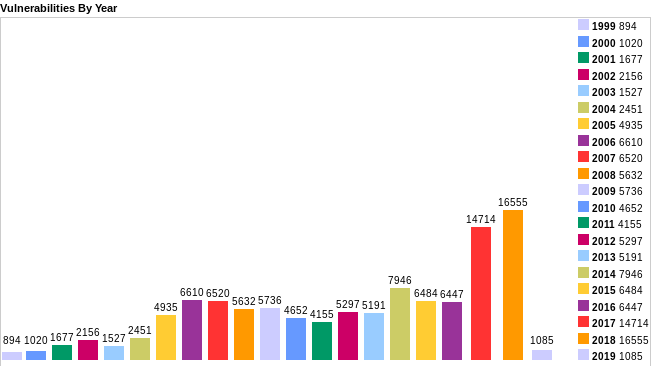
\includegraphics[scale=0.5]{img/cve_stats.png}
    }
    \caption{Статистика опубликованных уязвимостей за последние $20$ лет}
    \label{fig:image}
\end{figure}

Одним из популярных подходов к автоматизации поиска уязвимостей является фаззинг-тестирование \cite{DBLP:journals/corr/abs-1808-09700}. Это
техника тестирования программного обеспечения, заключающая в автоматической генерации входных данных. Целью фаззинга является нахождение таких входных данных, которые вызовут аварийное завершение программы.

Для достижения своей цели фаззеру необходимо генерировать входные данные, позволяющие пройти по разным путям выполнения. Один из популярных подходов, впервые примененный в AFL \cite{AFL} заключается в мутировании изначальных входных данных с целью увеличения покрытия.

Несмотря на высокую эффективность такого подхода он не лишен недостатков. Так например в листинге \ref{lst:example1}
\begin{lstlisting}[environoment=C_LANG, caption=example.c, captionpos=b, label={lst:example1}]
uint32_t buf[10];
read(10, &buf, 40);
buf[0] &= 500;

if (buf[0] == 100) {
    //branch 1
    ...
} else {
    //branch 2
    ...
}
\end{lstlisting}

для того, чтобы найти входные данные для прохождения по ветке $1$ необходимо фактически перебрать $2^{32}$ значений. Для решения подобных проблем в \cite{DRILLER} предлагается подход, основанный на динамическом символьном выполнении. В случае если фаззер не может сгенерировать входные данные для прохождения по некоторой ветке в течение некоторого ограниченного времени, запускается модуль символьного выполнения, который составляет и решает предикат пути. Затем фаззер продолжает свою работу.
Подход из \cite{DRILLER} реализован в инструменте \texttt{DRILLER}, распространяемом под открытой лицензией.

Комбинирование фаззинга и символьного выполнения тоже имеет свои сложности:
\begin{itemize}
    \item Генерация формул для каждой инструкции достаточно времязатратная операция.
    \item Задача поиска решений символьных уравнений является \textbf{NP полной}, не смотря на наличие множества эвристик невозможно гарантировать решение предиката пути за разумное время.
\end{itemize}

В данной работе предлагается иной способ улучшения эффективности открытия фаззером новых путей. В примере из листинга \ref{lst:example1} фаззер не знает от каких входных данных зависит условный переход и может мутировать все байты входного файла для открытия ветки $1$, однако в действительности значение \texttt{buf[0]} определяется только одним байтом, и только его и имеет смысл мутировать.
Так если у фаззера будет возможность для каждого условного перехода узнать от каких входных данных зависит его выполнение, это позволит существенно сократить количество итераций, необходимых для открытия пути.

Предметом работы является исследование и разработка методов, позволяющих предоставить фаззеру искомую информацию.

Целью работы является:
\begin{itemize}
    \item Исследовать методы динамического анализа с целью выявления подходов, применимых к задаче определения входных данных, влияющищих на выполнение условных переходов.
    \item Провести анализ существующих инструментов динамического анализа с точки зрения применимости к решаемой задаче.
    \item Разработать методы определения входных данных, влияющих на выполнение условных переходов на основе динамического символьного выполнения и на основе динамического анализа помеченных данных.
    \item Привести программную реализацию разработанных методов, провести её тестирование на наборе \texttt{LAVA} и программах с открытым исходным кодом.
\end{itemize}


В первой главе работы содержится обзор предметной области. Описываются предмет и методы динамического анализа. Дается обзор инструментов динамической бинарной инструментации, технологий динамического символьного выполнения и динамического анализа помеченных данных, а также существующих инструментов, использующих эти технологии.

Во второй главе описываются предлагаемые методы решения поставленной задачи.

В третьей главе проводится сравнение существующих инструментов с целью выбора базы для дальнейшей работы.

В четвертой главе описывается реализация предложенных методов.
